% ----------------------------------------------------------
\chapter{Fundamentação Teórica}\label{cap:fundamentacaoTeorica}
% ----------------------------------------------------------
Explicar brevemente o que será tratado como fundamentação teórica para o entendimento do contexto em que o modelo de aprendizagem de máquina será aplicado.

\section{As mudanças climáticas e as catástrofes naturais}

As grandes cidades brasileiras enfrentam desafios mais frequentes relacionados às mudanças climáticas, que agravam problemas como enchentes, inundações e deslizamentos. Projeções indicam que, até 2030, a mancha urbana de São Paulo pode aumentar em até 38\%, ampliando o risco para mais de 20\% das áreas de expansão urbana, que se tornarão suscetíveis a acidentes naturais (Nobre et al., 2011). O estudo também destaca que o aumento na frequência de eventos de chuvas intensas pode dobrar o número de dias com precipitação acima de 10 milímetros, agravando a vulnerabilidade da população, especialmente nas áreas periféricas e de menor infraestrutura.

\subsection{Cenário de enchentes no sul do Brasil}

Com base no histórico das enchentes no Rio Grande do Sul, observa-se que os desastres relacionados ao excesso de chuvas não são um fenômeno recente. Desde 1941, o estado lida com eventos catastróficos, como a enchente que devastou Porto Alegre naquele ano, considerada uma das mais graves da história da cidade. Ao longo das décadas, esses episódios continuaram a ocorrer, expondo a vulnerabilidade da região diante de chuvas intensas e repentinas. A combinação de fatores naturais, como a geografia da região e os ciclos climáticos, aliado as ações humanas nocivas ao meio ambiente, contribui para a repetição e intensificação dessas tragédias \cite{veja2024}.

Em Santa Catarina, estado adjacente ao Rio Grande do Sul, as enchentes também são fenômenos recorrentes que, ao longo dos anos, têm causado impactos sociais, econômicos e ambientais. Um dos eventos mais recentes foi registrado em maio de 2024, quando o estado registrou vários dias com altos indíces pluviométricos, levando ao transbordamento de rios, deslizamentos de terra e bloqueios em diversas rodovias \cite{g12024}.

\subsection{Dinâmica do Rio Guaíba}

O Rio Guaíba, principal manancial de abastecimento de água para a capital do Rio Grande do Sul e região, é alvo de estudo sobre diversos temas, incluindo sua hidrodinâmica e nível ao longo do ano. No Artigo conduzido pelos pesquisadores \cite{andrade2017}, a variabilidade nas descargas líquidas do Rio Guaíba revelou flutuações significativas nos volumes de descarga, variando de 407 m³/s a 14.270 m³/s, o que indica uma grande influência das condições climáticas sazonais e da vazão dos rios tributários, como o Jacuí, Taquarí, Caí e Sinos. Essas variações extremas foram observadas durante o período de 2014 a 2017 e reforçam a importância de monitorar continuamente o regime de águas do Guaíba para prevenir enchentes e outros desastres associados \cite{andrade2017}.

\section{Aprendizado de máquina}

Desde que os computadores foram inventados, criou-se o questionamento da possibilidade de fazê-los pensar de modo semelhante ao ser humano. Por meio desse avanço, diversas áreas sofreriam grandes transformações, uma vez que a capacidade da máquina aprender e aprimorar o seu conhecimento sobre determinado assunto traria melhorias e uma maior performance na atividade desejada \cite{carbonell1983}.

Embora os computadores ainda não alcancem o mesmo nível de aprendizado geral do ser humano, nos últimos anos, o aprendizado de máquina (do inglês, \textit{machine learning}, ou ML) se tornou realidade, com aplicações em diversos setores relacionados ou não a tecnologia, agregando valor e conhecimento por meio de dados e informações antes tratados apenas por profissionais da área.

Esse conceito envolve a criação de sistemas que são capazes de aprender a partir de dados, identificando padrões e realizando previsões sem a necessidade de programação explícita. De acordo com \cite{carbonell1983}, o principal objetivo do ML é construir algoritmos que permitam que os computadores adquiram conhecimento e melhorem sua performance de forma autônoma, baseando-se em experiências passadas.

\subsection{Categorias de aprendizado de máquina}

Com pesquisas e algoritmos sendo desenvolvidos para novas aplicações e/ou aprimoramento de implementações existentes, tornou-se necessário criar categorias de ML, a fim de classificar a sua função e estipular em quais cenários o seu uso é adequado.

Os quatro principais tipos de ML são: supervisionado, não supervisionado, semi-supervisionado e reforço \cite{saravanan2018}. 

\begin{itemize}
    \item Supervisionado: é o mais comum e envolve a utilização de dados rotulados, no qual o modelo é treinado com entradas e saídas conhecidas para fazer previsões sobre novos dados;
    \item Não supervisionado: lida com dados não rotulados, onde o sistema busca encontrar padrões ou agrupamentos nos dados;
    \item Semi supervisionado: combina elementos de ambos os métodos, utilizando uma pequena quantidade de dados rotulados e uma grande quantidade de dados não rotulados, sendo útil em cenários onde a rotulação de dados é cara ou complexa;
    \item Aprendizado por reforço: se baseia em um sistema de recompensas e punições, onde um agente interage com o ambiente e aprende a otimizar suas ações para alcançar um objetivo a partir de feedbacks recebidos.
\end{itemize}

\section{Regressão}

A partir da necessidade de realizar previsões, visando compreender e estimar a dinâmica dos fenômenos estudados, a regressão se apresenta como uma ferramenta que busca modelar relações entre variáveis dependentes e independentes através de métodos estatísticos \cite{soto2013}.

Em uma equação linear, uma variável independente, comumente representada pela letra $x$, caracteriza uma grandeza que está sendo manipulada durante um experimento. Dado esse comportamento, a variável $x$ não sofre influência de outras variáveis. A variável dependente, comumente representada pela letra $y$, caracteriza valores que estão diretamente associados à variável independente. Assim, de forma direta ou indireta, $x$ excerce influência sobre $y$.

Na Figura \ref{fig:regressao_exemplo}, a fim de exemplificar um caso de regressão, é apresentada a relação entre a expectativa de vida baseada e um índice de felicidade calculado em diversos países obtidos a partir de um levantamento feito por \cite{helliwell2020}. Neste estudo, a variável independente é representada pelo índice de felicidade, enquanto a expectativa de vida representa a variável independente. Desse modo, uma análise visual do gráfico permite inferir uma tendência de expectativa de vida maior em países com alto índice de felicidade. 

\begin{figure}[H]
	\caption{\label{fig:regressao_exemplo}Relação entre o índice de felicidade e expectativa de vida.}
	\begin{center}
		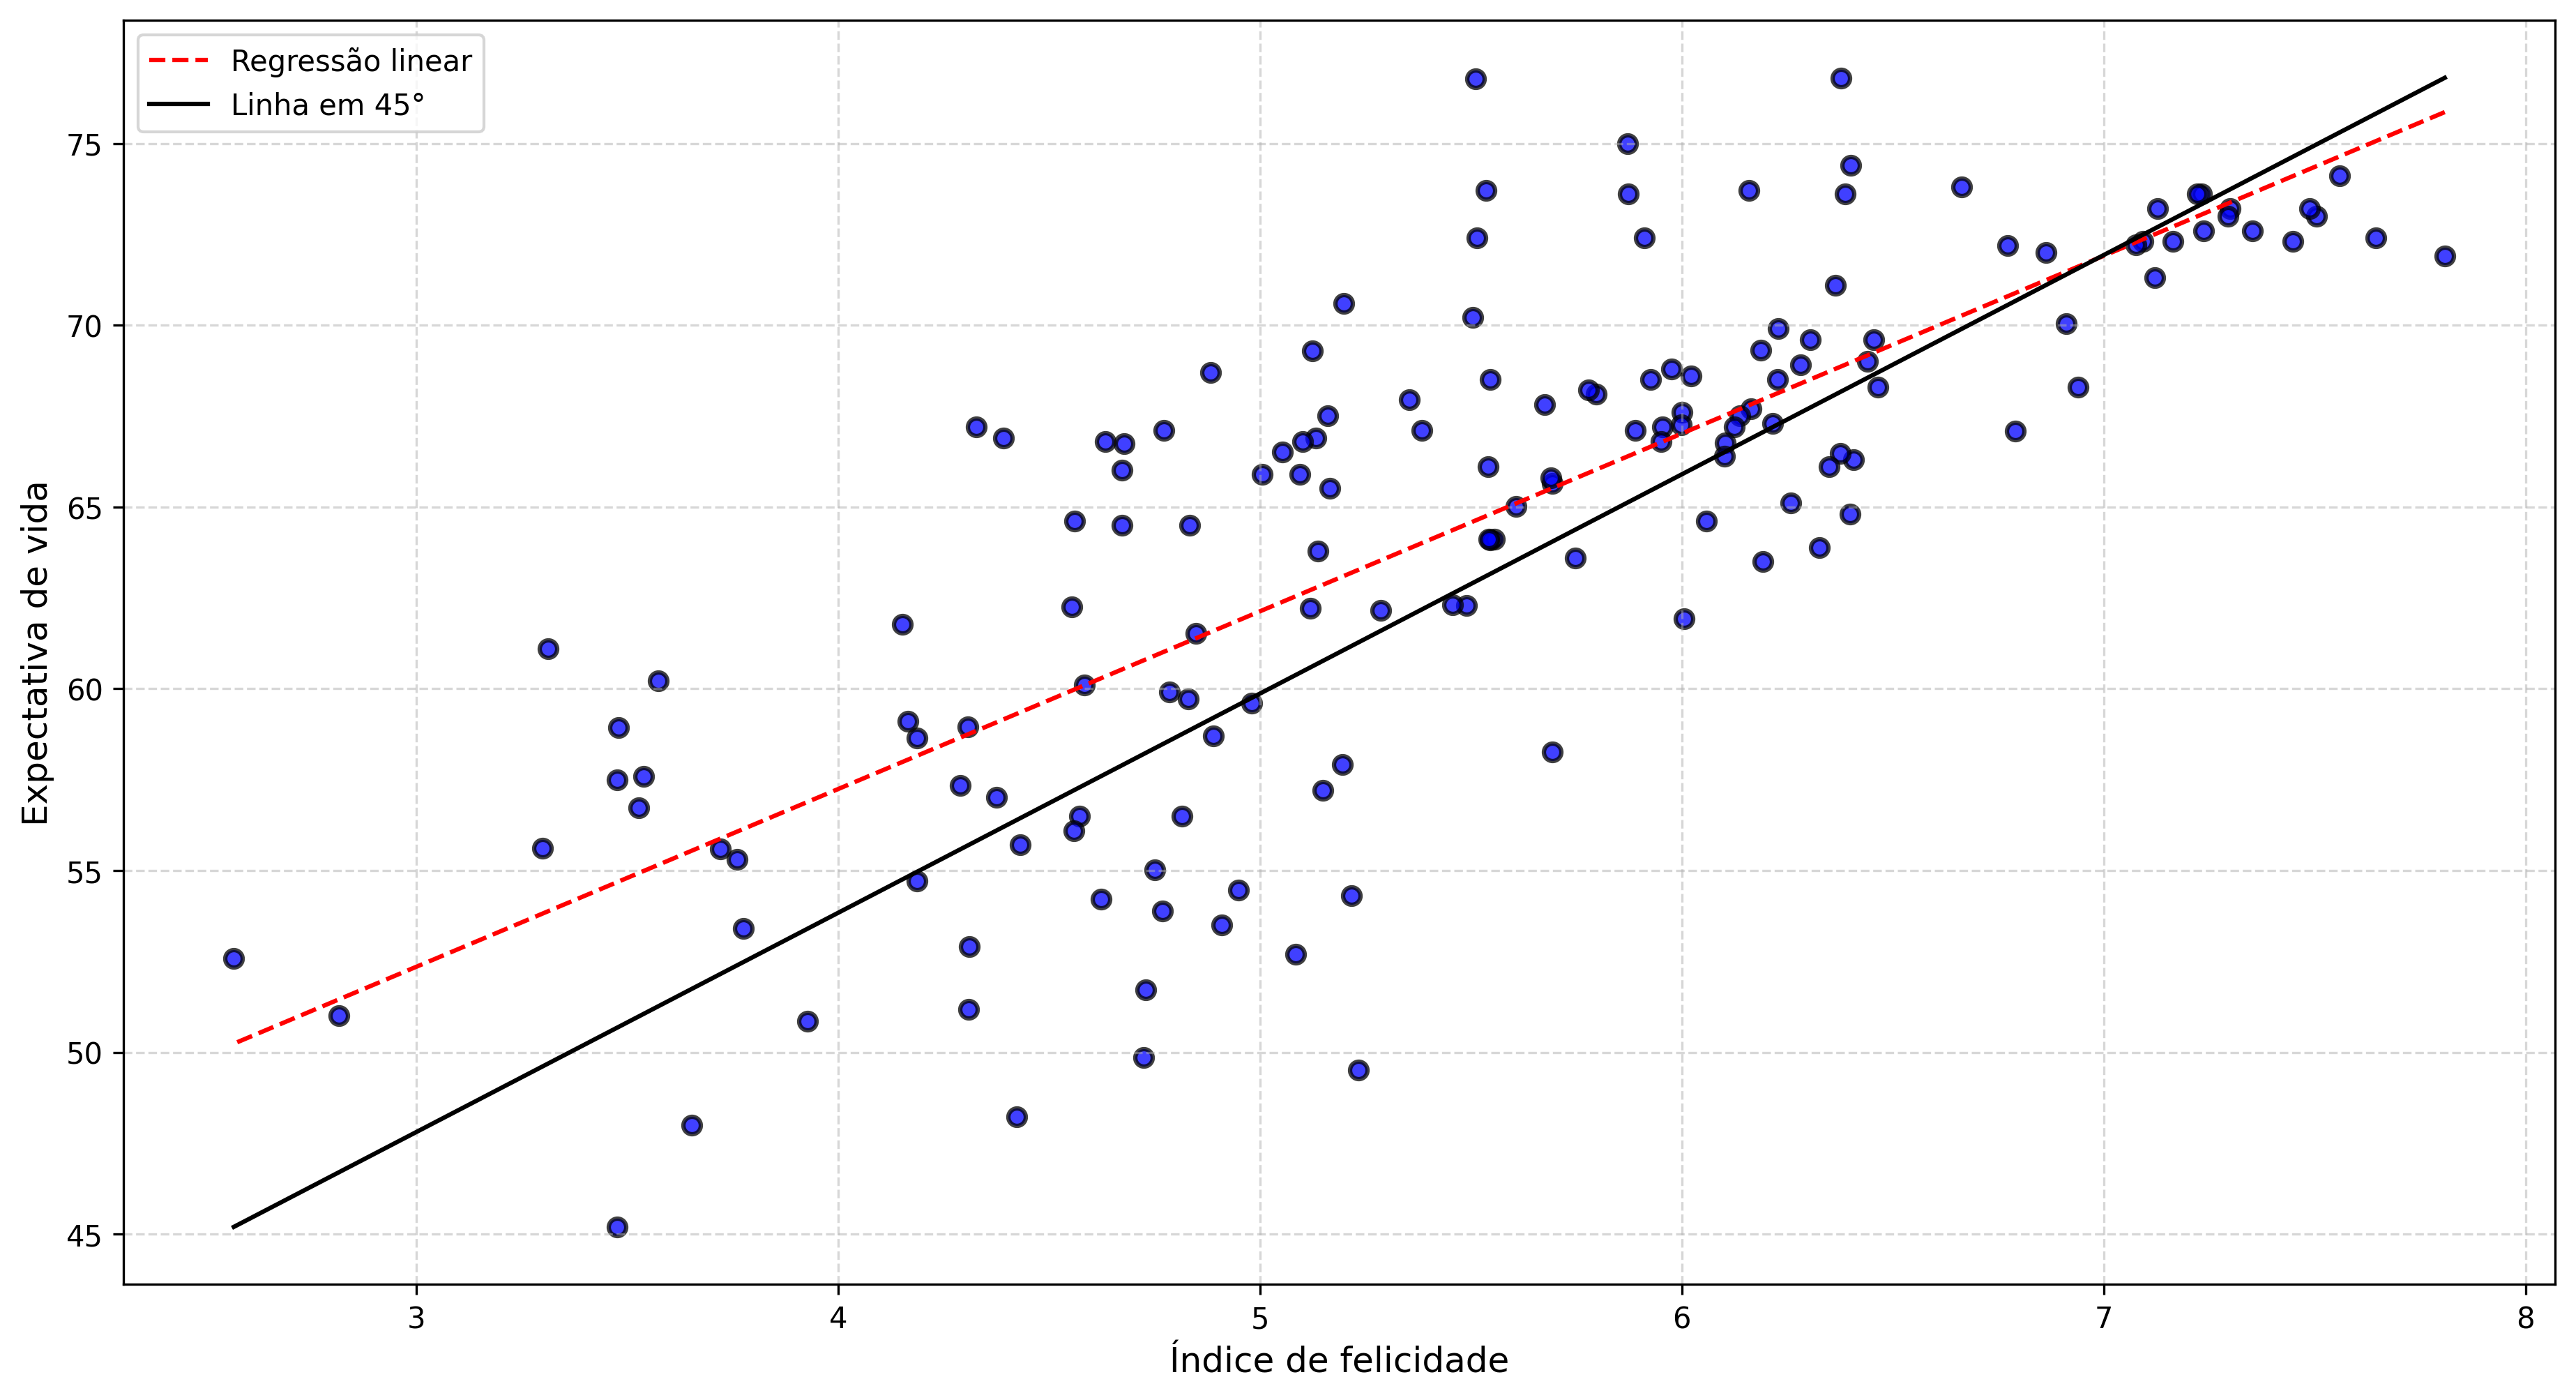
\includegraphics[scale=0.4]{figuras/happiness_world.png}
	\end{center}
	\fonte{\cite{helliwell2020}}
\end{figure}

Embora uma inferência inicial permita constatar uma correlação entre as váriavéis da equação, a criação de um modelo de previsão necessita de métodos que comprovem a correlação pressuposta. Para determinar as relações entre as variáveis dependentes e independentes de um sistema, coeficientes de correlação são calculados, gerando valores que medem e comprovam estatisticamente o grau de correspondência dos fatores estudados. Uma das métricas de correlação mais utilizadas é o coeficiente de Pearson, que mede a associação linear entre duas variáveis \cite{kirch2008}. 

Esse coeficiente de correlação pode ser definido pela Equação \ref{eq:correlacao_person}, onde $n$ é o total de amostras, $\bar{x}$ e $\bar{y}$ são as médias aritméticas de ambas as variáveis. Os valores do coeficiente de Pearson variam entre -1 e 1, de tal forma que quanto mais próximos desses extremos, melhor correlacionado estão as variáveis.

\begin{equation}
    r_{xy} = \frac{\sum_{i=1}^n (x_i - \bar{x})(y_i - \bar{y})}{\sqrt{\sum_{i=1}^n (x_i - \bar{x})^2 \sum_{i=1}^n (y_i - \bar{y})^2}}
    \label{eq:correlacao_person}
\end{equation}

A Figura \ref{fig:correlacoes} mostra alguns exemplos com gráficos de dispersão de variáveis com diferentes correlações.

\begin{figure}[H]
	\caption{\label{fig:correlacoes}Diferentes correlações entre variáveis.}
	\begin{center}
		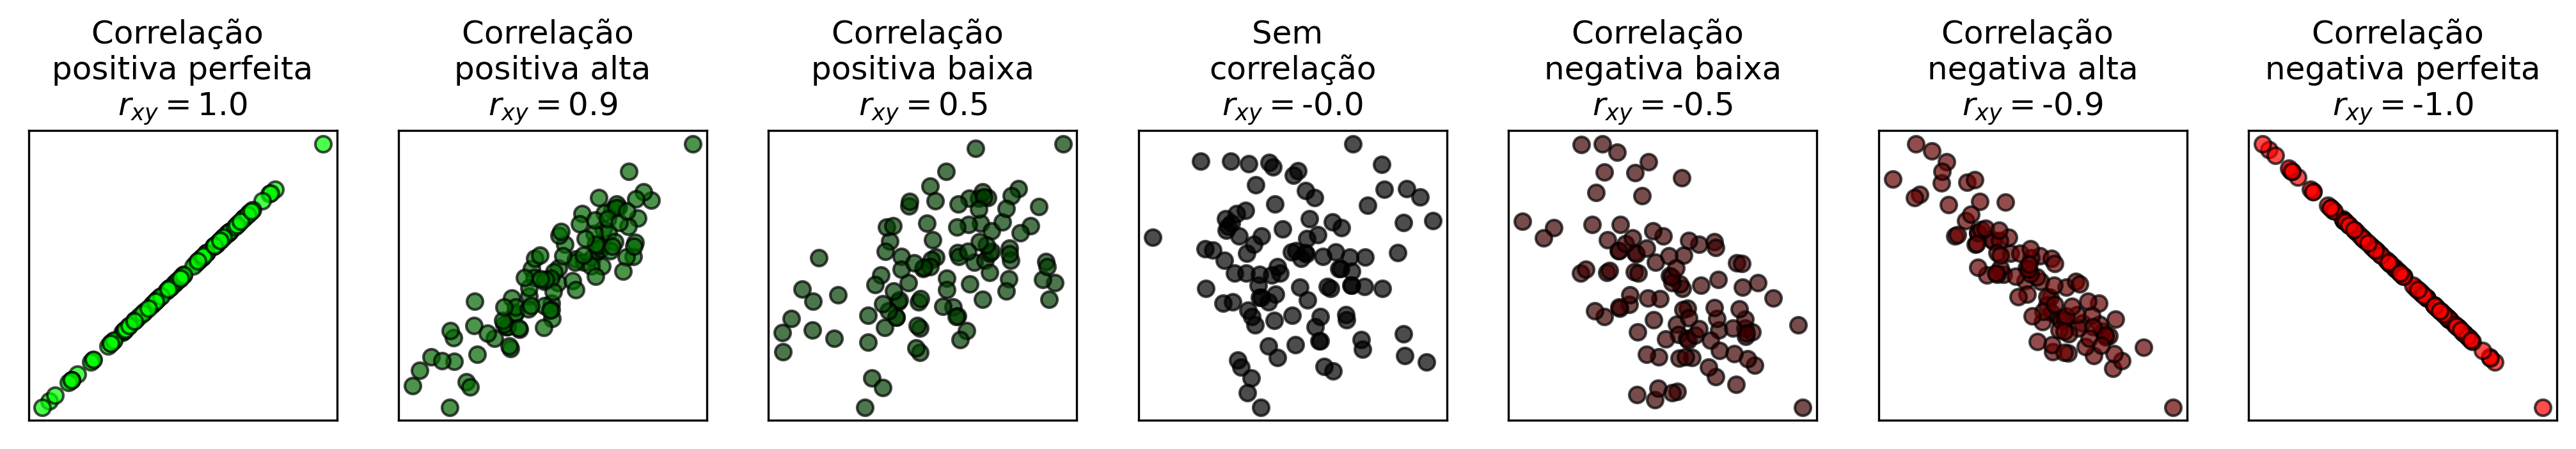
\includegraphics[scale=0.4]{figuras/correlations.png}
	\end{center}
	\fonte{\cite{helliwell2020}}
\end{figure}

Sendo assim, com o cálculo do coeficiente indicando uma alta correlação entre os dados estudados, os métodos de regressão utilizam esta premissa entre as variáveis para estimar valores não existentes no conjunto de dados. Contudo, o coeficiente de correlação também pode mostrar variáveis que não interferem na dinâmica uma da outra no conjunto de informações analisadas, tornando necessário o uso de algoritmos robustos, que dispensam esse o fator de correlação para realizar as previsões desejadas. 

\section{Regressão Linear}
\label{sec:regressao-linear}

A técnica de regressão linear é amplamente utilizada nos campos de estudo da engenharia, ciências físicas e químicas, economia, gestão, ciências biológicas e da vida, e ciências sociais. Em casos onde se deseja estabelcer uma relação entre uma variável preditora ou regressora (normalmente representada por $x$) e uma variável resposta (representada por $y$), a descrição dessa relação por meio de uma equação linear configura a implementação da técnica para a modelagem do problema estudado \cite{montgomery2012}.  

A aplicação da técnica é relevante devido à sua simplicidade e capacidade de fornecer previsões baseadas em uma fórmula matemática interpretável. Além disso, o método é base para implementações de algoritmos na área de ciência de dados como aprendizado de máquina, otimizando o processamento de dados complexos e viabilizando a criação de modelos de previsão \cite{aws2024}.

O método de regressão linear é dividido em dois grupos, sendo eles: regressão linear simples (RLS) e regressão linear múltipla (RLM) \cite{montgomery2012}. A RLS tem como objetivo estabelecer uma relação entre duas variáveis através de uma função, cuja definição é dada por:

\begin{equation}
	y = \beta_0 + \beta_1 x + \varepsilon
	\label{eq:regressao_linear_simples}
\end{equation}

Onde $y$ é a variável alvo, $x$ a variável regressora, enquanto $\beta_0$ e $\beta_1$ são coeficientes calculados pela regressão, que representam o intercepto no eixo Y e a inclinação da reta, respectivamente.

A RLM, embora seja semelhante à RLS, possui múltiplas variáveis preditoras, sendo definida por:

\begin{equation}
	y = \beta_0 + \beta_1 x_{1} + \beta_2 x_{2} + ... + \beta_k x_{k} + \varepsilon
	\label{eq:regressao_linear_multipla}
\end{equation}

Onde $y$ é a variável alvo, $x_{1}$ a $x_{k}$ as variáveis regressoras, e $\beta_0$ permanece sendo o coeficiente de intercepto do eixo Y enquanto $\beta_1$ a $\beta_n$ representam os coeficientes associados à n-ésima variável \cite{sassi2012}.

Em \ref{eq:regressao_linear_simples} e \ref{eq:regressao_linear_multipla}, nota-se a presença do erro estatístico representado por $\varepsilon$, que é a diferença entre o valor observado e o valor previsto pela equação de regressão. Esse erro é considerado aleatório e contabiliza a falha do modelo ao tentar se aproximar do comportamento denotado pelos dados amostrados \cite{montgomery2012}.

Partindo para um cenário ideal, a fim de se ter uma melhor compreensão do modelo de regressão linear, assume-se que seja possível fixar o valor da variável regressora $x$ ao observar um valor $y$ correspondente. Partindo dessa premissa, todos os valores do lado direito da equação \ref{eq:regressao_linear_simples} são conhecidos, exceto o erro $\varepsilon$, que passa a determinar as propriedades de $y$. Realizando outra suposição, onde a média e a variância de $\varepsilon$ são iguais a zero e $\sigma^2$, respectivamente \cite{montgomery2012}, a resposta média para qualquer valor da variável regressora é dada por:

\begin{equation}
	E(y \mid x) = \mu_{y \mid x} = E(\beta_0 + \beta_1x + \varepsilon) = \beta_0 + \beta_1x
\end{equation}

e a variância é dada por:

\begin{equation}
	Var (y \mid x) = \sigma_{y \mid x}^2 = Var(\beta_0 + \beta_1x + \varepsilon) = \sigma^2
\end{equation}

Desse modo, o modelo de regressão verdadeiro $\mu_{y \mid x} = \beta_0 + \beta_1x$ representa uma linha de valores médios, ou seja, a altura da linha de regressão em qualquer valor de x corresponde ao valor esperado de y para aquele x.

Para exemplificar a suposição acima, tem-se um modelo de regressão ilustrado pela Figura \ref{fig:observacoes_regressao_linear}, onde $\mu_{y \mid x} = 3,5 + 2x$, com variância $\sigma^2 = 2$. Nota-se que uma distribuição normal é utilizada para descrever a variação aleatória do erro $\varepsilon$. Estabelecido que $y$ é a soma de uma constante $\beta_0 + \beta_1x$ (a média) e uma variável aleatória normalmente distribuída, é possível inferir que $y$ também segue uma distribuição normal. No mesmo exemplo, se $x = 10$ amostras, $y$ terá distribuição normal com média $\mu_{y \mid x} = 3,5 + 2(10) = 23,5$ e variância $\sigma^2 = 2$. Quanto menor a variância, mais próximos os pontos estarão da linha de regressão, enquanto uma variância maior resultará em pontos mais dispersos em relação à linha de regressão \cite{montgomery2012}.

A maioria dos fênomenos nos quais se deseja obter a função que descreve o seu comportamento resulta em uma aproximação funcional através das variáveis de interesse. Essas relações funcionais frequentemente baseiam-se em teorias físicas, químicas ou de engenharia e ciências, ou seja, no conhecimento do mecanismo subjacente. Na Figura \ref{fig:regressao_linear_aprox_relacao_complexa}, é mostrada uma relação entre as variáveis $x$ e $y$ relativamente complexa, mas que pode ser aproximada de por uma equação de regressão linear, com um erro relativamente baixo.

\begin{figure}[H]
	\centering
	\caption{Interpretação de uma regressão linear}
	\begin{subfigure}{0.4\textwidth}
	  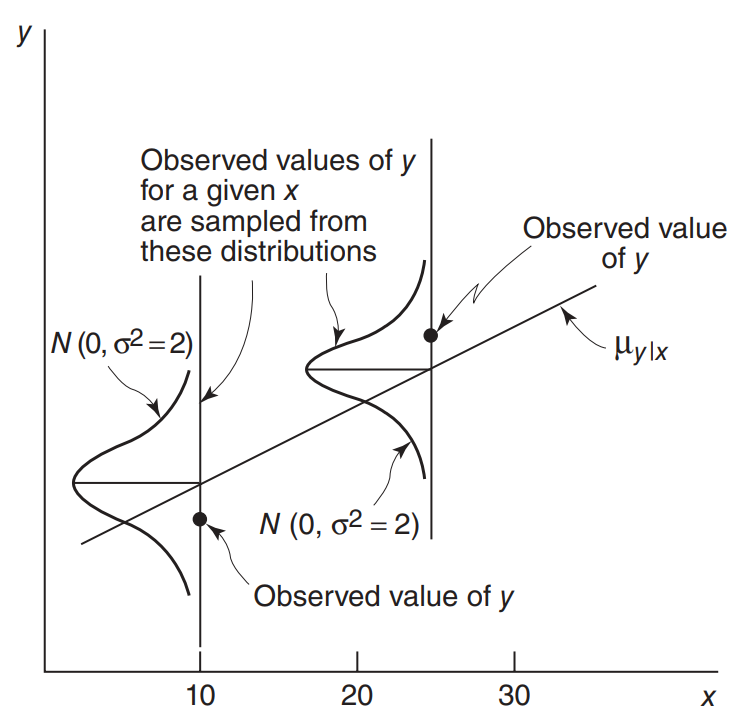
\includegraphics[width=\linewidth]{figuras/how_observations_are_generated_in_linear_regression.png}
	  \caption{Como as observações são geradas na regressão linear}
	  \label{fig:observacoes_regressao_linear}
	\end{subfigure}
	\hspace{0.5cm}
	\begin{subfigure}{0.4\textwidth} 
		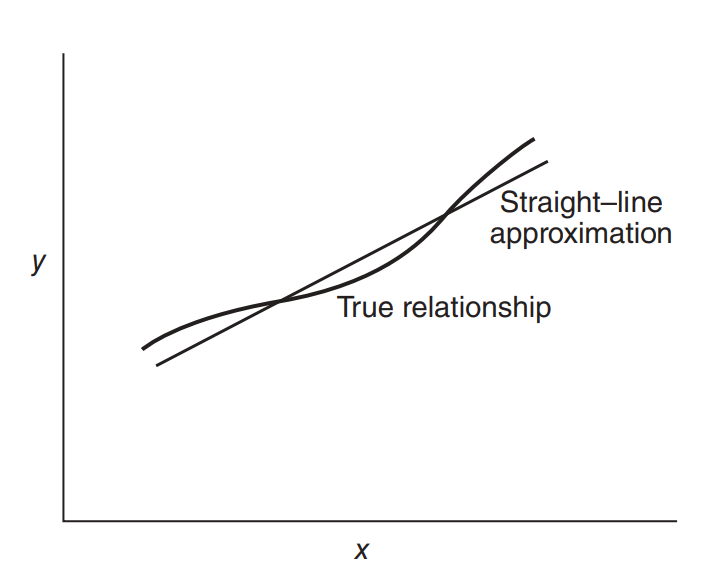
\includegraphics[width=\linewidth]{figuras/linear_regression_approximation_of_a_complex_relationship.png}
		\caption{Regressão linear como aproximação de uma relação complexa}
		\label{fig:regressao_linear_aprox_relacao_complexa}
	\end{subfigure}
	\label{fig:comportamento_regressao_linear}
	\fonte{\cite{montgomery2012}}
\end{figure}

Contudo, em alguns casos, quando a dinâmica do modelo a ser estimada passa a ter um grau de complexidade maior, como é o caso da Figura \ref{fig:aproximacao_linear_complexa}, utlizar uma RLS pode implicar em erros que extrapolam a tolerância exigida no estudo. Nesses cenários, utilizar uma função de regressão linear em intervalos específicos, ou seja, uma RLM, se torna uma alternativa plausível, tendo em vista que, para intervalos menores onde a dinâmica do fênômeno é mais linear, a regressão apresenta um erro menor, como mostra a Figura \ref{fig:intervalo_aplicacao_rls}.

\begin{figure}[H]
	\centering
	\caption{Situações de inadequação da RLS}
	\begin{subfigure}{0.4\textwidth}
	  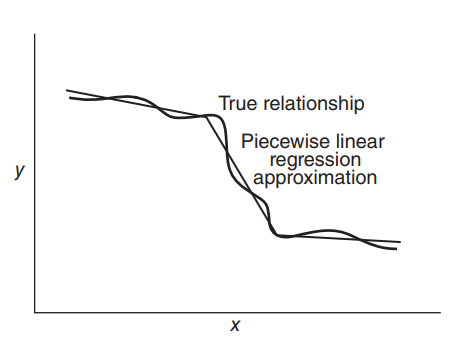
\includegraphics[width=\linewidth]{figuras/piecewise_linear_approximation.png}
	  \caption{Aproximação Linear complexa}
	  \label{fig:aproximacao_linear_complexa}
	\end{subfigure}
	\hspace{0.5cm}
	\begin{subfigure}{0.4\textwidth} 
		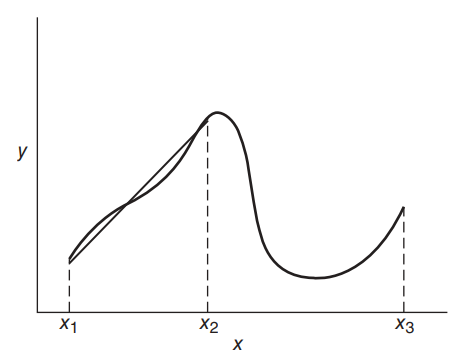
\includegraphics[width=\linewidth]{figuras/danger_extrapolation_regression.png}
		\caption{Intervalo de aplicação da RLS}
		\label{fig:intervalo_aplicacao_rls}
	\end{subfigure}
	\label{fig:comportamento_regressao_linear}
	\fonte{\cite{montgomery2012}}
\end{figure}

Partindo desses conceitos, para implementação de modelos de regressão linear e múltipla, o método dos Mínimos Quadrados Ordinários se apresenta como uma abordagem para estimar a melhor regressão dos pontos observados, encontrando uma reta com o menor erro entre as amostras e os valores da função estudada.

\section{Método dos quadrados ordinários}

O método dos Mínimos Quadrados Orinários (MQO) atua como uma ferramenta estatística, visando estimar a relação entre uma variável dependente e uma ou mais variáveis independentes \cite{Alkama2020}, permitindo encontrar os coeficientes desejados para o funcionamento do modelo.

Para obter uma regressão que se aproxima da dinâmica analisada, o método visa minimizar a Soma Residual dos Quadrados (RSS), denotado por:

\begin{equation}
	RSS = \sum_{i=1}^{n} \left(y_i - \beta_0 - \beta_1x_{i}\right)^2
\end{equation}

para os casos de RLS, ou seja, quando há apenas uma variável independente. Para o caso de RLM, a equação é dada por:

\begin{equation}
    RSS = \sum_{i=1}^{n} \left(y_i - \beta_0 - \sum_{j=1}^{p}\beta_jx_{ij}\right)^2
\end{equation}

onde:

\begin{itemize}
    \item $y_i$ é uma variável aleatória e representa o valor da variável resposta (variável dependente) na i-ésima observação
    \item $x_{ij}$ representa o valor da variável explicativa (variável independente, variável regressora) na i-ésima observação. Nota-se que podem existir múltiplas variáveis independentes para uma variável independente; 
    \item $\beta_{0}$ e $\beta_{j}$ são os parâmetros do modelo que serão estimados, e que definem a reta de regressão
\end{itemize}

Para minimizar a SSR em um caso de RLS, por exemplo, são calculadas as derivadas parciais de $\beta_0$ e $\beta_1$, igualando ambas a zero.

Derivada em relação à $\beta_0$:

\begin{equation}
	\frac{\partial SSR}{\partial \beta_0} = -2 \sum_{i=1}^n (y_i - \beta_0 - \beta_1 x_i) = 0
\end{equation}

simplificando:

\begin{gather*}
	\sum_{i=1}^n (y_i - \beta_0 - \beta_1 x_i) = 0 \\
	\sum_{i=1}^n y_i - n \beta_0 - \beta_1 \sum_{i=1}^n x_i = 0
\end{gather*}

divindindo por $n$:

\begin{gather*}
	\frac{\sum_{i=1}^n y_i}{n} - \beta_0 - \beta_1 \frac{\sum_{i=1}^n x_i}{n} = 0 \\
	\bar{y} - \beta_0 - \beta_1 \bar{x} = 0
\end{gather*}

onde $\bar{y}$ e $\bar{x}$ são as médias amostrais de $y$ e $x$, respectivamente. Assim, a equação pode ser reescrita como:

\begin{equation}
	\beta_0 = \bar{y} - \beta_1 \bar{x}
	\label{eq:beta0}
\end{equation}

Derivada em relação à $\beta_1$:

\begin{equation}
	\frac{\partial SSR}{\partial \beta_1} = -2 \sum_{i=1}^n x_i (y_i - \beta_0 - \beta_1 x_i) = 0
\end{equation}

substituindo $\beta_0$ na equação:


\begin{gather*}
	\sum_{i=1}^n x_i (y_i - (\bar{y} - \beta_1 \bar{x}) - \beta_1 x_i) = 0 \\
	\sum_{i=1}^n x_i (y_i - \bar{y} + \beta_1 \bar{x} - \beta_1 x_i) = 0 \\
	\sum_{i=1}^n x_i (y_i - \bar{y}) + \sum_{i=1}^n x_i (\beta_1 \bar{x} - \beta_1 x_i) = 0 \\
	\sum_{i=1}^n x_i (y_i - \bar{y}) - \beta_1 \sum_{i=1}^n x_i (x_i - \bar{x}) = 0
\end{gather*}

sabendo que:

\begin{gather*}
	\sum_{i=1}^n x_i (x_i - \bar{x}) = \sum_{i=1}^n (x_i - \bar{x})^2
\end{gather*}

e

\begin{gather*}
	\sum_{i=1}^n x_i (y_i - \bar{y}) = \sum_{i=1}^n (x_i - \bar{x})(y_i - \bar{y})	
\end{gather*}

portanto:

\begin{gather*}
	\sum_{i=1}^n (x_i - \bar{x})(y_i - \bar{y}) = \beta_1 \sum_{i=1}^n (x_i - \bar{x})^2
\end{gather*}

\begin{equation}
	\beta_1 = \frac{\sum_{i=1}^n (x_i - \bar{x})(y_i - \bar{y})}{\sum_{i=1}^n (x_i - \bar{x})^2}
\end{equation}




Desse modo, a partir de um problema onde uma ou mais entradas geram amostras que resultam em uma saída, torna-se possível estimar uma função que melhor representa seu comportamento, minimizando ao máximo o valor da soma residual dos quadrados entre os pontos amostrais e a curva do modelo. 

\begin{table}[h!]
\centering
\begin{tabular}{|c|c|}
\hline
\textbf{Variável Independente} & \textbf{Variável Dependente} \\
\hline
0,38 & 6,98 \\
0,41 & 4,05 \\
0,44 & 5,52 \\
0,59 & 6,93 \\
0,98 & 6,57 \\
1,04 & 6,41 \\
1,22 & 8,27 \\
1,53 & 6,93 \\
1,74 & 8,89 \\
1,84 & 9,31 \\
\hline
\end{tabular}
\caption{Tabela de Valores Ordenados: Variável Independente vs. Variável Dependente}
\label{tab:valores_exemplo_mqo}
\end{table}

A Tabela \ref{tab:valores_exemplo_mqo} apresenta um exemplo de dados amostrais, onde a variável independente é representada pela primeira coluna e a variável dependente pela segunda coluna. A partir desses dados, é possível aplicar o método dos mínimos quadrados para encontrar os coeficientes que melhor se ajustam à reta de regressão linear.

Ao aplicar o método para resolver um problema, como é o caso da Tabela \ref{tab:valores_exemplo_mqo}, todos os pontos amostrados são utilizados para encontrar a reta que melhor se ajusta aos dados. Contudo, visando mostrar como a dinâmica de regressão utilizando MQO funciona, nos passos seguintes, as amostras são consideradas de forma cumulativa, alterando a cada iteração os valores de $\beta_0$ e $\beta_1$, até que a reta de regressão linear se ajuste aos dados amostrais.

Passo 1: Apenas o ponto (0.44, 5.52)

Com um único ponto, a reta passa exatamente por sobre o mesmo, porém o método MQO exige pelo menos dois pontos para definir uma inclinação. Assim, assume-se uma reta horizontal ao usar o ponto como base inicial.

\begin{gather*}
	\beta_0 = 5.52, \quad \beta_1 = 0
\end{gather*}


\begin{figure}[H]
	\caption{\label{fig:mqo_1}Passo 1 da regressão linear pelo método MQO.}
	\begin{center}
		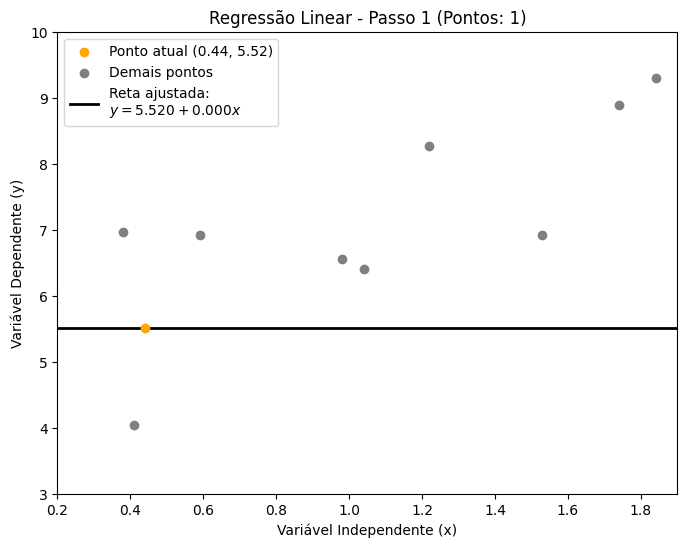
\includegraphics[scale=0.5]{figuras/RL_step_1.png}
	\end{center}
	\fonte{Autor.}
\end{figure}

Passo 2: Adiciona-se (1.74, 8.89)
\\
n=2

\begin{gather*}
	\bar{x} = \frac{0.44 + 1.74}{2} = 1.09, \quad \bar{y} = \frac{5.52 + 8.89}{2} = 7.205 \\
	\sum (x_i - \bar{x})(y_i - \bar{y}) = (0.44 - 1.09)(5.52 - 7.205) + (1.74 - 1.09)(8.89 - 7.205) = \\ 
	(-0.65)(-1.685) + (0.65)(1.685) = 1.09525 + 1.09525 = 2.1905 \\
	\sum (x_i - \bar{x})^2 = (0.44 - 1.09)^2 + (1.74 - 1.09)^2 = 0.4225 + 0.4225 = 0.845 \\
	\beta_0 = \frac{2.1905}{0.845} \approx 2.5923\\
	\beta_1 = 7.205 - 2.5923 \cdot 1.09 \approx 7.205 - 2.8255 = 4.3795\\ \\
	\hat{y} = 4.3795 + 2.5923x
\end{gather*}

\begin{figure}[H]
	\caption{\label{fig:mqo_2}Passo 2 da regressão linear pelo método MQO.}
	\begin{center}
		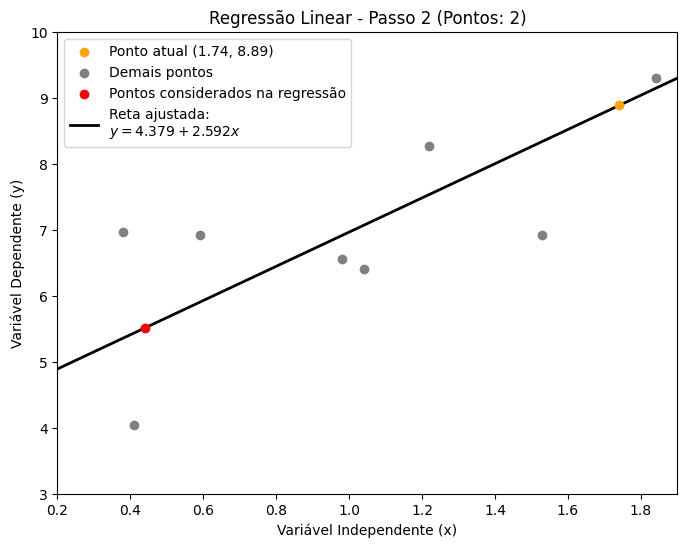
\includegraphics[scale=0.5]{figuras/RL_step_2.png}
	\end{center}
	\fonte{Autor.}
\end{figure}

Passo 3: Adiciona (0.41, 4.05)
\\ n = 3

\begin{gather*}
	\bar{x} = \frac{0.44 + 1.74 + 0.41}{3} = 0.8633, \quad \bar{y} = \frac{5.52 + 8.89 + 4.05}{3} = 6.1533 \\
	\sum (x_i - \bar{x})(y_i - \bar{y}) = \\ 
	(0.44 - 0.8633)(5.52 - 6.1533) + \\
	(1.74 - 0.8633)(8.89 - 6.1533) + \\
	(0.41 - 0.8633)(4.05 - 6.1533) \approx  \\
	0.268 + 2.399 + 0.953 = 3.62 \\ \\
	\sum (x_i - \bar{x})^2 = (0.44 - 0.8633)^2 + (1.74 - 0.8633)^2 + (0.41 - 0.8633)^2 \\
	\approx 0.179 + 0.769 + 0.205 = 1.153 \\
	\beta_0 = \frac{3.62}{1.153} \approx 3.1402 \\
	\beta_1 = 6.1533 - 3.1402 \cdot 0.8633 \approx 6.1533 - 2.711 = 3.4423 \\ \\
	\hat{y} = 3.4423 + 3.1402x
\end{gather*}

\begin{figure}[H]
	\caption{\label{fig:mqo_2}Passo 3 da regressão linear pelo método MQO.}
	\begin{center}
		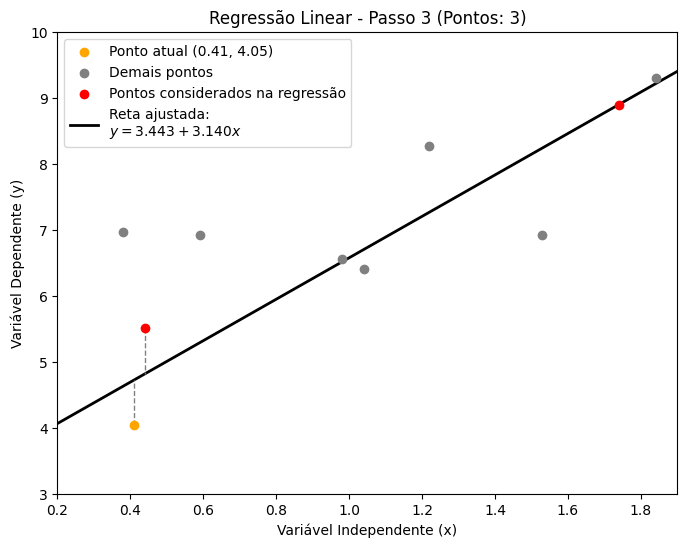
\includegraphics[scale=0.5]{figuras/RL_step_3.png}
	\end{center}
	\fonte{Autor.}
\end{figure}

Para os demais passos, o mesmo cálculo é realizado, onde a média amostral e os coeficientes são recalculados a cada iteração, conforme os pontos são adicionados.

\begin{figure}[H]
	\centering
	\caption{Iterações da aplicação do método MQO}
	\begin{subfigure}{0.4\textwidth}
	  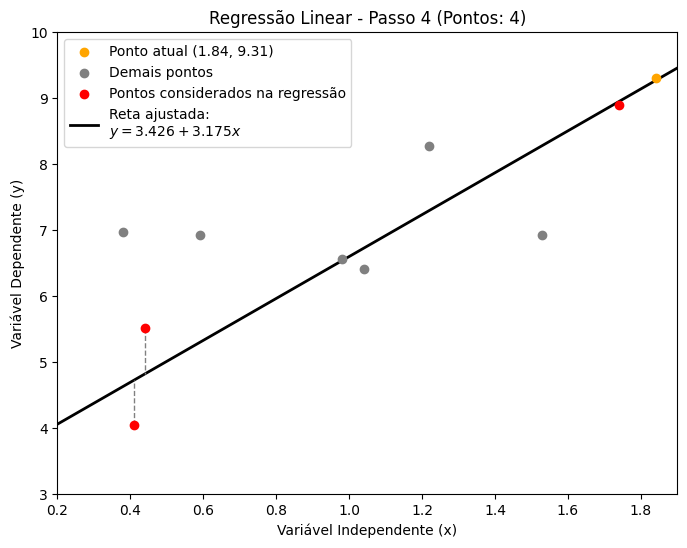
\includegraphics[width=\linewidth]{figuras/RL_step_4.png}
	  \caption{$n = 4$ | $y = 3,426 + 3,175x$}
	  \label{fig:mqo_4}
	\end{subfigure}
	\hspace{0.5cm}
	\begin{subfigure}{0.4\textwidth} 
		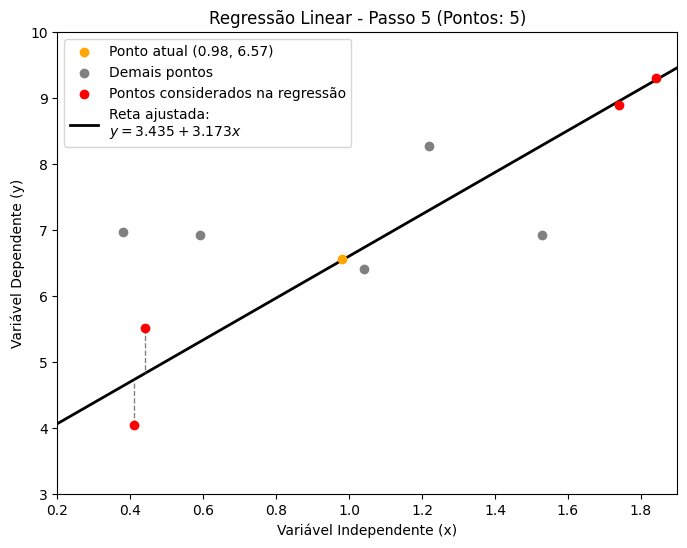
\includegraphics[width=\linewidth]{figuras/RL_step_5.png}
		\caption{$n = 5$ | $y = 3,435 + 3,173x$}
		\label{fig:intervalo_aplicacao_rls}
	\end{subfigure}
	\label{fig:mqo_5}
	\begin{subfigure}{0.4\textwidth} 
		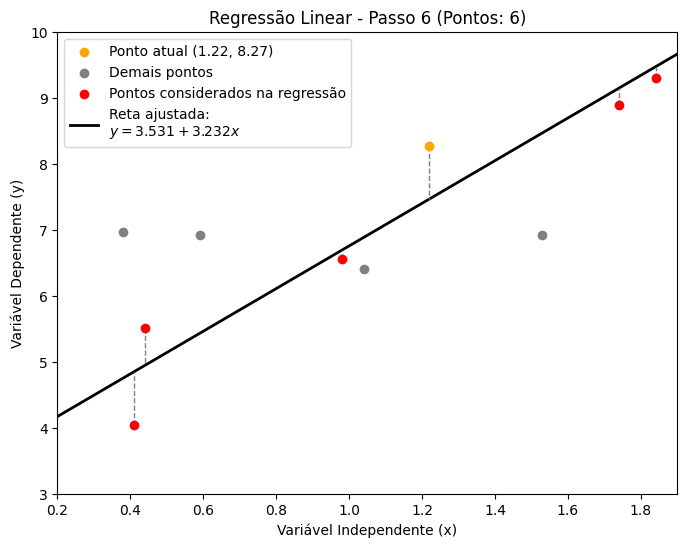
\includegraphics[width=\linewidth]{figuras/RL_step_6.png}
		\caption{$n = 6$ | $y = 3,531 + 3,232x$}
		\label{fig:intervalo_aplicacao_rls}
	\end{subfigure}
	\label{fig:mqo_6}
	\begin{subfigure}{0.4\textwidth} 
		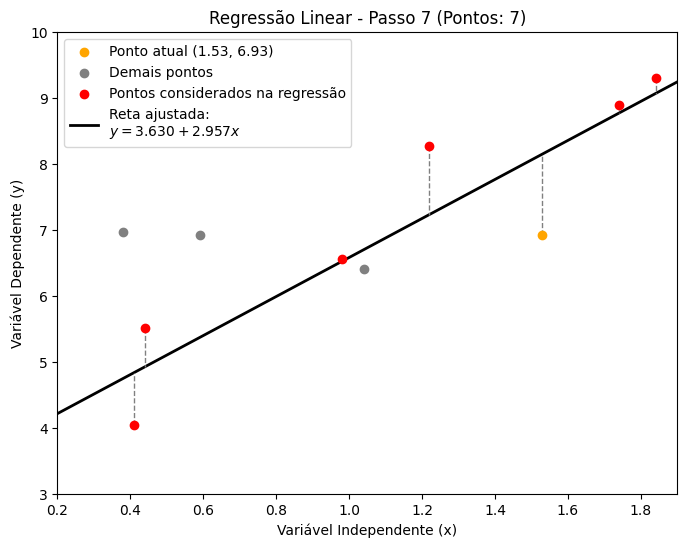
\includegraphics[width=\linewidth]{figuras/RL_step_7.png}
		\caption{$n = 7$ | $y = 3,630 + 2,957x$}
		\label{fig:intervalo_aplicacao_rls}
	\end{subfigure}
	\label{fig:mqo_7}
	\begin{subfigure}{0.4\textwidth} 
		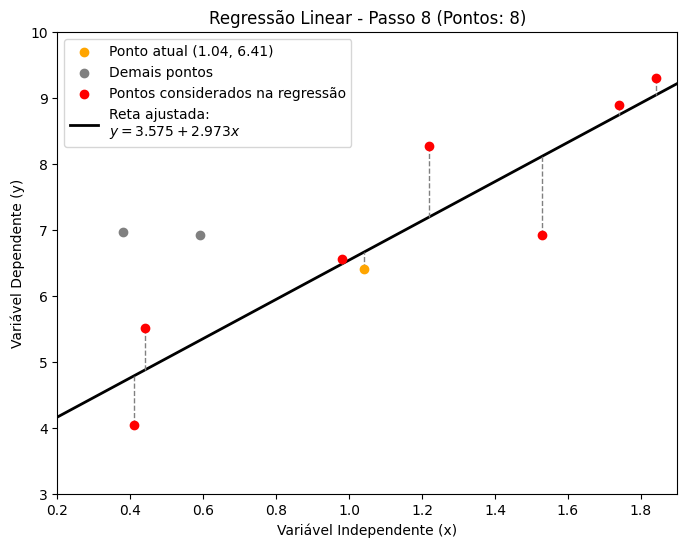
\includegraphics[width=\linewidth]{figuras/RL_step_8.png}
		\caption{$n = 8$ | $y = 3,575 + 2,973x$}
		\label{fig:intervalo_aplicacao_rls}
	\end{subfigure}
	\label{fig:mqo_8}
	\begin{subfigure}{0.4\textwidth} 
		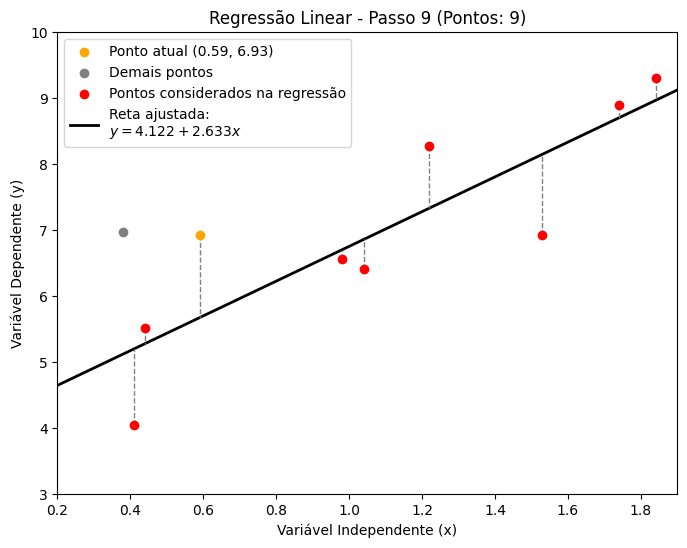
\includegraphics[width=\linewidth]{figuras/RL_step_9.png}
		\caption{$n = 9$ | $y = 4,122 + 2,633x$}
		\label{fig:intervalo_aplicacao_rls}
	\end{subfigure}
	\label{fig:mqo_9}
	\fonte{Autor.}
\end{figure}

Assim, a cada ponto selecionado da amostra, é calculada a derivada parcial da função estimada, determinando novos coeficiente que melhor descrevem a reta entre as amostras. Dado que não é possível estimar uma reta que passe sobre todos os pontos amostrados, os resíduos representados pelas linhas tracejadas na Figura \ref{fig:mqo_10} são definidos de tal modo que o somatório dos seus quadrados seja o menor possível.


\begin{figure}[H]
	\caption{\label{fig:mqo_10}Passo 10 da regressão linear pelo método MQO.}
	\begin{center}
		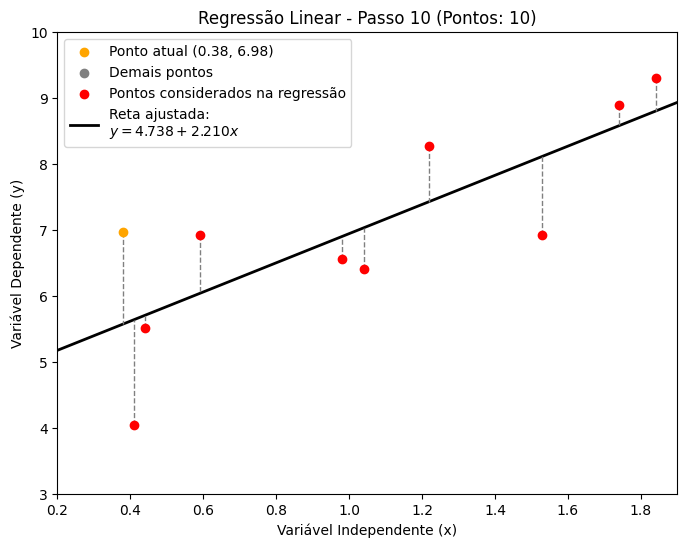
\includegraphics[scale=0.6]{figuras/RL_step_10.png}
	\end{center}
	\fonte{Autor.}
\end{figure}


\section{Modelo Ridge}

A Regressão Ridge é uma técnica de regularização estatística amplamente utilizada em modelos de regressão linear para abordar problemas de sobreajuste (overfitting) e multicolinearidade entre variáveis preditoras \cite{McDonald:2009:RR}. Essa técnica, também conhecida como regularização L2, é particularmente eficaz em cenários onde o número de variáveis preditoras é grande ou quando essas variáveis apresentam alta correlação, o que pode levar a estimativas de coeficientes instáveis e de baixa generalização.

Conforme visto em \ref{sec:regressao-linear}, na regressão linear tradicional, o objetivo é minimizar a soma dos quadrados dos resíduos (Residual Sum of Squares, RSS), que mede a diferença entre os valores observados e os valores previstos pelo modelo. A função de perda é dada por:

\begin{equation}
	RSS = \sum_{i=1}^{n} (y_i - \hat{y}_i)^2
\end{equation}

onde $y_i$ são os valores observados, $\hat{y}_i$ são os valores previstos, e $n$ é o número de observações. No entanto, em cenários com multicolinearidade (alta correlação entre variáveis preditoras) ou um grande número de preditores, o modelo pode se ajustar excessivamente aos dados de treinamento, resultando em alta variância e baixa performance em dados não vistos. A Regressão Ridge resolve esse problema ao adicionar um termo de penalidade à função de perda, proporcional à soma dos quadrados dos coeficientes de regressão. 

A função objetivo da Regressão Ridge é:

\begin{equation}
	RSS_{L2} = \sum_{i=1}^{n} (y_i - \hat{y}_i)^2 + \lambda \sum_{j=1}^{p} \beta_j^2
\end{equation}

No contexto da biblioteca \textit{Scikit-learn} em Python, a classe Ridge implementa a regressão ridge. O parâmetro alpha define a força da regularização: valores maiores de $\lambda$ resultam em coeficientes mais próximos de zero, enquanto valores menores permitem que o modelo se aproxime da regressão linear ordinária. A escolha adequada de 
$\lambda$ é crucial para evitar tanto o overfitting  (quando o modelo se ajusta demais aos dados de treinamento) quanto o underfitting (quando o modelo é muito simples para capturar os padrões dos dados). \cite{ScikitLearnRidge2025}.

% O modelo Ridge, implementado na biblioteca \textit{scikit-learn} do Python, é uma variação da regressão linear de MQO que incorpora um termo de regularização L2 à função de custo, o que ajuda a controlar a complexidade do modelo e prevenir o sobreajuste (\textit{overfitting}), ou seja, o treinamento de um modelo que não é capaz de realizar previsões em outros cenários, exceto aquele que lhe foi passado no treinamento \cite{ScikitLearnRidge2025}. Com essa caracterísica, o método é indicado em casos onde os dados apresentam colinearidade ou onde há muitas variáveis independentes \cite{Jolly2018}.

% \begin{equation}
% 	J(\beta) = \sum_{i=1}^{n} (y_i - \hat{y}_i)^2 + \alpha \sum_{j=1}^{p} \beta_j^2
% \end{equation}

% No primeiro termo, observa-se o somatório dos erros quadráticos, semelhante ao método MQO. No segundo termo, é aplicada a penalização L2, que é a soma dos quadrados dos coeficientes do modelo, multiplicada por um hiperparâmetro $\alpha$ que controla a intensidade da regularização. O valor de $\alpha$ deve ser ajustado para encontrar o equilíbrio entre o ajuste do modelo e a complexidade do mesmo \cite{ScikitLearnRidge2025}.

%  A regressão linear padrão visa minimizar a soma dos erros quadráticos (Erro Quadrático Médio ou MSE) entre as previsões e os valores reais. No entanto, em casos onde o dataset apresenta muitos recursos ou quando os dados apresentam correlações entre as variáveis, o modelo tende a se ajustar demais aos dados de treinamento (\textit{overfitting}). A fim de contornar tal problema, o modelo Ridge adiciona um termo de penalidade à função de custo, que regula o tamanho dos coeficientes do modelo. Esse comportamento é observado na função de custo do modelo, com a adição de um hiperparâmetro $\lambda$ em relação ao modelo de regressão linear padrão.

% \begin{equation}
%     J(\theta) = \frac{1}{m}\sum_{i=1}^{m}\left(h_{\theta}(x^{(i)})- y^{(i)}\right)^2 + \lambda\sum_{j=1}^{n}\theta^{2}_{j}
% \end{equation}

% onde:

% \begin{itemize}
%     \item $\lambda$ é o hiper-parâmetro que controla a intensidade da regularização;
%     \item $\theta_{j}$ são os coeficientes (ou pesos) do modelo;
%     \item Quanto maior o valor de $\lambda$, maior será a penalização para grandes coeficientes, resultando em um modelo mais simples.
% \end{itemize}

% Sendo assim, a inclusão do termo somado a equação de regressão linear padrão reduz a magnitude dos coeficientes, ajudando a controlar o \textit{overfitting}. Em essência, o modelo Ridge evita que o modelo aprenda padrões específicos do conjunto de treinamento que não se generalizam bem para dados novos.



